\documentclass[10pt]{exam}
\usepackage[utf8]{inputenc}		% Caracteres latinos
\usepackage[spanish]{babel}		% Idioma español
\usepackage{geometry}			% Organizar el documento
\usepackage{graphicx}			% Incluir gráficos
\usepackage{makecell}			% Para personalizar las celdas de una tabla
\usepackage[nohdr]{mathexam}	% Añadimos el paquete mathexam (sin header)
\usepackage{amsmath}
\usepackage{amsfonts}
\usepackage{amssymb}
\usepackage{mathtools}
\usepackage{tikz,pgfplots}
\usepgfplotslibrary{polar}
 \renewcommand{\baselinestretch}{1.5}

%\usepackage[]{mathptmx}        % A free version o Times Roman with mathematical symbols
%\usepackage{pzc}               % fuente cursiva (conjuntos) Zapf Chancery
%\usepackage{showframe}
%\usepackage{lipsum}

% DOCUMENTACIÓN DE LA CLASE EXAM
% http://ftp.inf.utfsm.cl/pub/tex-archive/macros/latex/contrib/exam/examdoc.pdf
% DOCUMENTACIÓN DE LA CLASE MATHEXAM
% http://ctan.dcc.uchile.cl/macros/latex/contrib/mathexam/doc/mathexam.pdf

% Definimos la geometría de la primera página
\geometry{
	a4paper,                    % Tamaño del documento
	hmargin = {1.5cm, 1.0cm}, 	% Margen horizontal izquierdo, derecho
	vmargin = {0.8cm, 1cm},	    % Margen vertical superior, inferior
	headsep = 4mm,				% Separación entre el encabezado y el texto
	head = .2cm,				% Tamaño del encabezado
	% marginparsep = 5mm, 		% Seperación entre las notas y el texto
	% marginpar = 1.5cm,		% Tamaño de las notas
	includeall,                 % incluye el encabezado, footer y notas dentro del tamaño del documento
	nomarginpar,	            % Elimina las notas
	foot = 1cm,                 % Tamaño del footer
	twoside,                	% Habilita el modo de impresión a doble cara
}

\selectlanguage{spanish}        % Selecciona el idioma
\spanishdecimal{.}

%\pagestyle{headandfoot}         % Nuestro examen tendrá encabezado y pié

% DEFINIMOS EL ENCABEZADO
%\header{
%\begin{tabular}{l c c c l}
%            \makecell{\includegraphics[height=2.5cm]{logo.png}} &
%            \makecell{\textbf{IPEA 215} \\Raúl Scalabrini Ortiz} &
%            \makecell{Examen} &
%            \makecell{Curso\\1er Año} &
%             \makecell[l]{Apellido y %Nombre:\enspace\makebox[2in]{\hrulefill}\\Fecha: \today}
%        \end{tabular}}{}{}

% DEFINIMOS EL PIE
%\rfoot{Página \thepage\ de \numpages}

% DOCUMENTO
\begin{document}

\centering


\Large 
\textbf{Tarea 1}

\normalsize
Fecha de entrega: 

% 23/08/2019 durante la clase
Martes 03/09/2024 durante la clase



\pointpoints{punto}{puntos}
\pointformat{\bfseries\boldmath(\thepoints)}
\vskip10pt
%$\frac{1}{p}+\frac{1}{q}=\frac{1}{f}$

%$\frac{1}{20}+\frac{1}{q_1}=\frac{1}{10}\Rightarrow\frac{1}{q_1}=\frac{1}{10}-\frac{1}{20}\Rightarrow q_1=20$

%$\frac{1}{5}+\frac{1}{q_2}=\frac{1}{20}\Rightarrow\frac{1}{q_2}=\frac{1}{20}-\frac{1}{5}\Rightarrow q_2=-6.666$

%$d(l_1,l_2)=25$


\begin{questions}
    \question Sea $\mathcal{X}$ el conjunto que denota a todas las personas. ¿Cuál de las siguientes reglas de correspondencia definen una función $\mathcal{X}\rightarrow\mathcal{X}$? Explica porqué.
    \begin{parts}
    \part $f(\textbf{\textit{a}})$ es la madre de $\textbf{\textit{a}}$.
    \part $g(\textbf{\textit{a}})$ es el mejor amigo de $\textbf{\textit{a}}$.
    \part $h(\textbf{\textit{a}})$ es el hermano de $\textbf{\textit{a}}$.
    \part $k(\textbf{\textit{a}})$ es el primero hijo o hija de $\textbf{\textit{a}}$ si $\textbf{\textit{a}}$ tiene hijos, y es su padre si $\textbf{\textit{a}}$ no tiene hijos.
    \end{parts}
    

    \question ¿Cuáles de los siguientes diagramas representan funciones? ¿Porqué? ¿En que casos el codominio coincide con la imagen de la función? \vskip20pt
    
    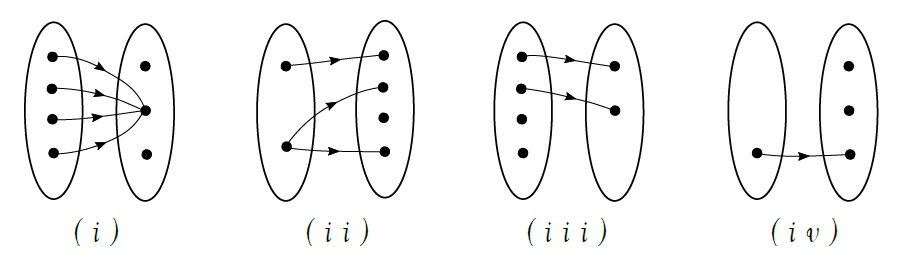
\includegraphics[scale=0.9]{Func1.jpg}
    
    \question Para cada una de las siguientes reglas de asignación, encuentra el dominio de la función; es decir, el subconjunto más grande $\mathcal{X}\subseteq\mathbb{R}$ tal que $g:\mathcal{X}\rightarrow\mathbb{R}$ es una función. Determina su imagen y si se trata de un función par, impar o ninguna de las dos. 
    \begin{parts}
    \part $f(x)=\sqrt{x^2-4}\,,\quad x\in\mathcal{X}$
   % \part $g(x)=\frac{1}{x^4-3}\,,\quad x\in\mathcal{X}$
   \part $f(x)=e^{-x^2}$
   \part $f(x)=e^{senx}$
    \end{parts}
    
    \question Define las reglas de correspondencia de las siguientes funciones y determina el dominio de la función resultante para: a) $f+g$, b) $f+g$, c) $fg$, d) $f/g$, e) $g/f$.   
    \begin{itemize}
        \item $f(x)=\sqrt{x},\quad g(x)=x^2+1$
        \item $f(x)=\dfrac{x+1}{x-1},\quad g(x)=\dfrac{1}{x}$
    \end{itemize}

    %\newpage
    \question Decide que tipo de función modela los datos en las siguientes gráficas de dispersión. Explica tu elección.
    \begin{center}
        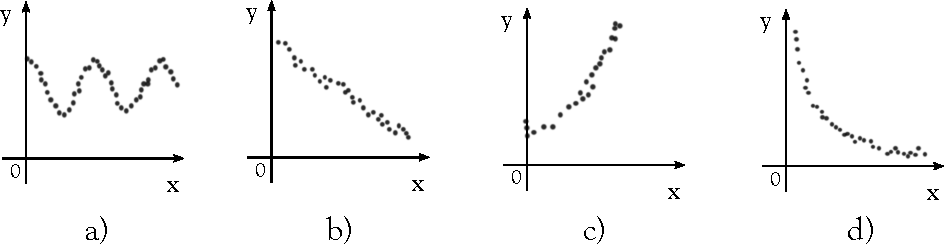
\includegraphics[scale=1]{grafdisp.pdf}
    \end{center}
    
    % \question Se desea descongelar un pastel en un horno calentándolo durante 1 hr. Transcurrido este tiempo se sacas y se deja enfriar, antes de comerlo.
    % Describe como cambia la temperatura del pastel conforme pasa el tiempo . Traza una gráfica aproximada de la temperatura del pastel como función del tiempo.
    \question Determina si los números $-1$ y $2$ están en el rango de la función racional $f(x)=\dfrac{2x-1}{x+4}$.

    \question Una pelota es lanzada hacia arriba desde el nivel del suelo con una velocidad inicial de $96\, ft/s$. La altura de la pelota desde el suelo está dada por la función cuadrática $s(t)=-16t^2+96t$. ¿En qué momentos la pelota está en el suelo? Grafica $s(t)$ sobre el intervalo para el cual $s(t)\geq0$.

  %  \question A menudo se supone que el peso $W$ de un cuerpo es función de su longitud $L$. Esta suposición está dada por la función de potencia $W=kL^3$, donde $k$ es una constante. Para un cierto lagarto, $k=400\,g/m^3$. Determina el peso si su longitud es de $0.5\,m$.
    
    \question Estudios recientes indican que la temperatura superficial de la Tierra se ha incrementando de manera constante. Algunos científicos han modelado la temperatura mediante la función lineal $T=0.02t+8.50$, donde $\textbf{\textit{T}}$ es la temperatura en $^{\circ}C$ y $\textbf{\textit{t}}$ representa los años transcurridos desde 1900:
    
    \begin{parts}
    \part¿Qué representa la pendiente y la ordenada al origen de ésta función lineal?
    \part Utiliza la ecuación para predecir la temperatura superficial global promedio en el año 2100.
    \end{parts}

    % \question Los chirridos de cierta especie de grillo están relacionados con la temperatura de forma "casi lineal". Un individuo de esta especie produce 103 chirridos por minutos a una temperatura de $50^{\circ}C$ y 183 a $70^{\circ}F$:
    % \begin{parts}
    % \part[1/3] ¿Cuál es la ecuación que modela la temperatura en función del número de chirridos por minuto?
    % \part[1/3] ¿Que representa la pendiente en esta ecuación y cuál es su valor?
    % \part[1/3] ¿A que temperatura esta el ambiente si un grillo emite 155 chirridos por minutos?
    % \end{parts}

    \question En cada caso, determina una función como un modelo matemático del problema particular.
    \begin{itemize}
        \item El peso aproximado del cerebro de una persona es directamente proporcional al peso de su cuerpo, y una persona que pesa 150 lb tiene un cerebro cuyo peso aproximado es de 4 lb. Encuentra un modelo matemático que exprese el peso aproximado del cerebro como una función del peso de la persona y posteriormente determina el peso aproximado del cerebro de una persona que pesa 176 lb. 
        \item En un lago, un pez grande se alimenta de un pez mediano y la población del pez grande es una función $f$ de $x$, el número de peces de tamaño mediano en el lago. A su vez, el pez mediano se alimenta de un pez pequeño, y la población de peces medianos es una función $g$ de $w$, el número de peces pequeños en el lago. Sean $$f(x)=\sqrt{20x}+150, \quad \quad g(w)=\sqrt{w}+5000$$
        Encuentra un modelo matemático que exprese la población de peces grandes como una función del número de peces pequeños en el lago. Determina el número de peces grandes cuando el lago contiene 9 millones de peces pequeños.
    \end{itemize}

    \question Expresa la función $F(x)=\dfrac{1}{\sqrt{x+\sqrt{x}}}$ como una composición de 3 funciones.
    
    \end{questions}


% Geometría para la otra carilla
\newgeometry{
	hmargin = {1.5cm, 1.5cm},
	vmargin = {1.5cm, 1.5cm},
	%nofoot,			% Elimina el pié
	nohead,			% Elimina el encabezado
	nomarginpar,	% Elimina las notas
	includeall,
}% \savegeometry{geometria_1}

\pagestyle{foot}    % El estilo de ésta página sólo constará de pié de página
\runningfooter{}{}{Página \thepage\ de \numpages}


%\lipsum[1-5]

% \restoregeometry
% \loadgeometry{geometria_1}


\end{document}
